% Provenance (never printed): see sources/outline_sources.md (Year 1: heat sources,
% radiogenic and secular cooling; heat-flow measurement; the steady conductive geotherm
% with heat production; convection against conduction; the lithosphere as a thermal
% boundary layer). Curves from figdata/bachelor-1/geotherms.py; exercise and problem
% values in the Book 3 scratch calculator calc/ch10.py.
\chapter{El balance térmico de la Tierra}\label{ch:b1:heat-budget}

Bajo una montaña de los Alpes japoneses, en una antigua cavidad minera, un tanque con mil toneladas de centelleador líquido
vigila destellos de luz muy débiles. La mayoría procede de antineutrinos producidos en los reactores nucleares del país de
alrededor, pero algunos vienen de abajo: el uranio y el torio del interior de la Tierra emiten antineutrinos al desintegrarse,
y estos atraviesan todo el planeta como si estuviera vacío. En 2135 días de recuento el detector registró 841 sucesos
candidatos, de los que 106 se atribuyeron a la propia Tierra. A partir de ese puñado de destellos, su equipo estimó en 2011 que
la desintegración del uranio y el torio calienta la Tierra con unos 20 teravatios. El planeta en conjunto pierde unos 47. Este
capítulo explica la diferencia: de dónde procede el calor de la Tierra, cómo se mide el calor que sale de ella, cómo sube la
temperatura con la profundidad cuando el calor se transporta por conducción, por qué el \omterm{def:b1:layered-earth:layers}{manto} debe convectar, y por qué las
placas son la frontera superior y fría de esa convección.

\begin{recall}
El calor fluye de lo caliente a lo frío; la conductividad térmica $k$ de una roca mide lo fácilmente que el calor la atraviesa, y
la difusividad térmica $\kappa = k/(\rho c)$, lo deprisa que se extiende un cambio de temperatura (física, segundo año
universitario). Los núcleos radiactivos se desintegran con una semivida fija (física). La temperatura sube con la profundidad a lo
largo del \omterm{def:b1:heat-budget:geotherm}{geotermo}, y el \omterm{def:b1:layered-earth:layers}{manto} convecta (libro 2, años 11 y 12). La \omterm{def:b1:layered-earth:lithosphere}{litosfera} es la cáscara exterior resistente de la Tierra
(\cref{ch:b1:layered-earth}).
\end{recall}

\section{De dónde viene el calor}

\begin{definition}[Flujo de calor]\label{def:b1:heat-budget:heat-flow}
El \emph{flujo de calor}\index{flujo de calor} $q$ en un punto de la superficie de la Tierra, o densidad de flujo de calor
superficial, es la potencia de origen interno que atraviesa la superficie allí, por unidad de área, contada positiva hacia
fuera. Se mide en \unit{W.m^{-2}}, en la práctica en \unit{mW.m^{-2}}. Integrado sobre toda la superficie, da la pérdida de
calor de la Tierra $Q = \oint q\,\mathrm dS$.
\end{definition}

El \omterm{def:b1:heat-budget:heat-flow}{flujo de calor} se ha medido en decenas de miles de lugares. Una recopilación de \num{38347} medidas, publicada en 2010,
da los valores medios siguientes, contando por separado los océanos y los continentes:
\begin{center}
\small
% ledger: dd10:split, dd10:total
\begin{tabular}{lccc}
\hline
 & superficie (\unit{m^2}) & pérdida de calor (\unit{TW}) & \omterm{def:b1:heat-budget:heat-flow}{flujo de calor} medio (\unit{mW.m^{-2}}) \\
\hline
continentes & \num{2.073e14} & 14.7 & 70.9 \\
océanos & \num{3.028e14} & 31.9 & 105.4 \\
Tierra entera & \num{5.101e14} & 46.7 & 91.6 \\
\hline
\end{tabular}
\end{center}
El total, redondeado a su incertidumbre, es $Q = \qty[uncertainty-mode=separate]{47 \pm 2}{TW}$. Dos tercios de él salen por el
fondo oceánico, que es más joven y más delgado que los continentes. Es un flujo pequeño: el Sol entrega a la Tierra unos
\qty{173000}{TW}, y el calor interno representa el \qty{0.03}{\percent} del balance de energía en la superficie. % ledger: nasa:solar-mean
Pero es el flujo que impulsa los volcanes, las placas y la formación de montañas, y tiene dos fuentes.

\begin{definition}[Producción de calor radiogénico]\label{def:b1:heat-budget:heat-production}
La \emph{producción de calor radiogénico}\index{producción de calor radiogénico} $A$ de una roca es el calor liberado por unidad
de volumen y de tiempo por la desintegración de los núcleos radiactivos que contiene, en \unit{W.m^{-3}}, en la práctica en
\unit{\micro W.m^{-3}}. Una roca de densidad $\rho$ que contiene fracciones másicas $C_i$ de los elementos productores de calor,
cada uno de los cuales libera $H_i$ vatios por kilogramo de elemento, tiene
\[
  A = \rho \sum_i C_i H_i .
\]
\end{definition}

Cuatro isótopos producen casi todo este calor, porque son de vida larga, suficientemente abundantes y energéticos:
\ce{^{238}U}, \ce{^{235}U}, \ce{^{232}Th} y \ce{^{40}K}. El calor por kilogramo de cada elemento es el calor por kilogramo de su
isótopo radiactivo multiplicado por la proporción de ese isótopo en el elemento (\cref{exo:b1:heat-budget:3}):
\begin{center}
\small
% ledger: dye:isotope-heat, iaea:isotopes
\begin{tabular}{lcccc}
\hline
isótopo & semivida & calor por kg de isótopo & proporción del & calor por kg de elemento \\
 & (\unit{Gyr}) & (\unit{W.kg^{-1}}) & elemento (átomos) & (\unit{W.kg^{-1}}) \\
\hline
\ce{^{238}U} & 4.468 & \num{9.513e-5} & \qty{99.274}{\percent} & U: \num{9.85e-5} \\
\ce{^{235}U} & 0.704 & \num{5.685e-4} & \qty{0.720}{\percent} & \\
\ce{^{232}Th} & 14.0 & \num{2.628e-5} & casi todo & Th: \num{2.63e-5} \\
\ce{^{40}K} & 1.248 & \num{2.847e-5} & \qty{0.0117}{\percent} & K: \num{3.40e-9} \\
\hline
\end{tabular}
\end{center}
El potasio libera treinta mil veces menos calor por kilogramo que el uranio, pero es un elemento principal de muchas rocas,
contado en tanto por ciento, mientras que el uranio y el torio se cuentan en partes por millón. Las rocas ricas en los tres son
los granitos y sus parientes; las más pobres son las peridotitas del \omterm{def:b1:layered-earth:layers}{manto}. Una recopilación de \num{2188} análisis da estas
medianas, en \unit{\micro W.m^{-3}}:
\begin{center}
\small
% ledger: vila:heat-production
\begin{tabular}{lclclc}
\hline
riolita & 2.55 & lutitas & 1.44 & gabro & 0.35 \\
granito & 2.43 & areniscas & 0.82 & basalto & 0.21 \\
granodiorita & 1.88 & rocas carbonatadas & 0.42 & rocas ultramáficas & 0.11 \\
\hline
\end{tabular}
\end{center}
La dispersión dentro de cada grupo es grande: un cuarto de los granitos produce menos de \qty{1.74}{\micro W.m^{-3}}, un cuarto
más de \qty{3.23}{\micro W.m^{-3}}. La \omterm{def:b1:layered-earth:layers}{corteza} continental está enriquecida en estos elementos, y la \omterm{def:b1:layered-earth:layers}{corteza} oceánica y el \omterm{def:b1:layered-earth:layers}{manto}
empobrecidos; pero el \omterm{def:b1:layered-earth:layers}{manto} es tan grande que aún contiene una gran parte de las fuentes de calor del planeta.

\begin{definition}[Enfriamiento secular]\label{def:b1:heat-budget:secular-cooling}
El \emph{enfriamiento secular}\index{enfriamiento secular} es la parte de la pérdida de calor de la Tierra suministrada por la lenta
disminución de la temperatura de su interior, \omterm{def:b1:layered-earth:layers}{manto} y núcleo: la liberación del calor almacenado desde la formación del planeta,
a un ritmo $-\sum_j M_j c_j\,\mathrm dT_j/\mathrm dt$ para depósitos de masa $M_j$, calor específico $c_j$ y temperatura media $T_j$.
\end{definition}
La conservación de la energía da el balance de toda la Tierra: el calor perdido en la superficie es la producción radiogénica más el
\omterm{def:b1:heat-budget:secular-cooling}{enfriamiento secular},
\[
  Q = H_{\text{rad}} + Q_{\text{sc}} .
\]
Los geoneutrinos miden una parte del primer término: el resultado de 2011, que combinó dos detectores, atribuye \qty{20}{TW} al
uranio y al torio, y se sabe que el \ce{^{40}K}, cuyos antineutrinos son demasiado débiles para detectarse así, añade unos
\qty{4}{TW}.
% ledger: kamland:2011
Alrededor de la mitad de la pérdida de calor es, por tanto, radiogénica, y la otra mitad, unos \qty{23}{TW}, es \omterm{def:b1:heat-budget:secular-cooling}{enfriamiento
secular}. Parte de ese enfriamiento es del núcleo: el calor que atraviesa la \omterm{def:b1:layered-earth:discontinuity}{frontera núcleo--manto} se estima en
\qtyrange{5}{15}{TW}. Estas cifras son inciertas: la medida misma tiene una incertidumbre de unos \qty{9}{TW}, y los resultados
de los geoneutrinos hasta ahora solo acotan la parte radiogénica entre \qtyrange{15}{41}{TW}, mientras que los modelos de Tierra
de distintos tipos varían entre \qtyrange{14}{46}{TW}. El total, medido en la superficie, es el término mejor conocido del balance
(figura siguiente).
% ledger: dye:radiogenic

\begin{omfigure}
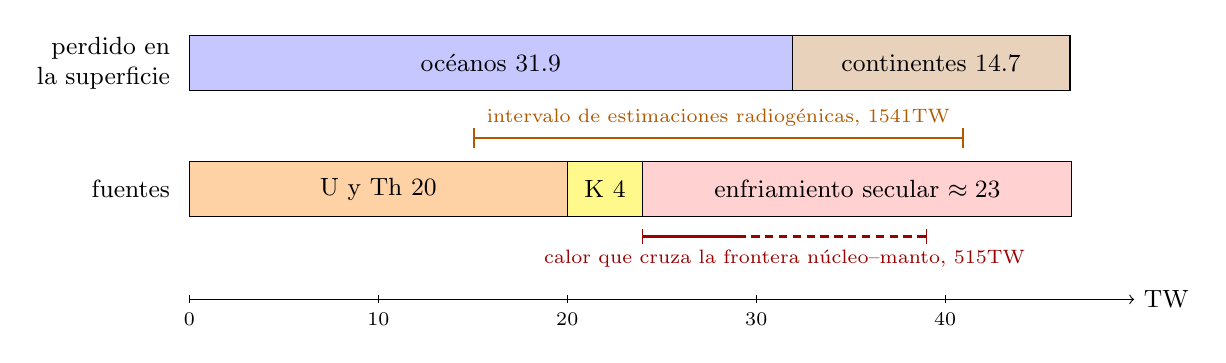
\begin{tikzpicture}[x=0.24cm, y=1cm, font=\small]
% ledger: dd10:split, kamland:2011, dye:radiogenic
% losses
\fill[blue!22] (0,1.6) rectangle (31.9,2.3);
\fill[brown!35] (31.9,1.6) rectangle (46.6,2.3);
\draw (0,1.6) rectangle (46.6,2.3);
\draw (31.9,1.6) -- (31.9,2.3);
\node at (15.95,1.95) {océanos 31.9};
\node at (39.25,1.95) {continentes 14.7};
\node[anchor=east, align=right, font=\small] at (-0.5,1.95) {perdido en\\la superficie};
% sources
\fill[orange!35] (0,0) rectangle (20,0.7);
\fill[yellow!45] (20,0) rectangle (24,0.7);
\fill[red!18] (24,0) rectangle (46.7,0.7);
\draw (0,0) rectangle (46.7,0.7);
\draw (20,0) -- (20,0.7) (24,0) -- (24,0.7);
\node at (10,0.35) {U y Th 20};
\node at (22,0.35) {K 4};
\node at (35.35,0.35) {enfriamiento secular $\approx 23$};
\node[anchor=east, align=right] at (-0.5,0.35) {fuentes};
% core part of secular cooling (range)
\draw[red!60!black, very thick] (24,-0.25) -- (29,-0.25);
\draw[red!60!black, thick, densely dashed] (29,-0.25) -- (39,-0.25);
\draw[red!60!black] (24,-0.15) -- (24,-0.35) (39,-0.15) -- (39,-0.35);
\node[anchor=north, font=\scriptsize, red!60!black] at (31.5,-0.3) {calor que cruza la frontera núcleo--manto, \qtyrange{5}{15}{TW}};
% radiogenic range
\draw[|-|, orange!70!black, thick] (15,1.0) -- (41,1.0);
\node[anchor=south, font=\scriptsize, orange!70!black] at (28,1.02) {intervalo de estimaciones radiogénicas, \qtyrange{15}{41}{TW}};
% axis
\draw[->] (0,-1.05) -- (50,-1.05) node[right] {TW};
\foreach \x in {0,10,20,30,40} {\draw (\x,-1.0) -- (\x,-1.1) node[below, font=\scriptsize] {\x};}
\end{tikzpicture}

\par\smallskip{\small El presupuesto térmico de la Tierra. Arriba: el calor perdido a través del fondo
oceánico y de los continentes, \qty[uncertainty-mode=separate]{47 \pm 2}{TW} en total. Abajo: sus fuentes,
con la parte radiogénica del uranio y del torio medida con geoneutrinos y la del potasio estimada; el resto,
por diferencia, es \omterm{def:b1:heat-budget:secular-cooling}{enfriamiento secular}, del que el núcleo aporta una parte mal conocida. La barra naranja
muestra el intervalo de la parte radiogénica permitido por las medidas de geoneutrinos.}
\label{fig:b1:heat-budget:budget}
\end{omfigure}

Las fuentes radiogénicas fueron mayores en el pasado, porque los isótopos eran más abundantes:
\ce{^{235}U} y \ce{^{40}K}, los de vida corta, contribuían entonces mucho más (libro 2, año 12). El motor térmico
de la Tierra se apaga despacio, por ambas causas.

\section{Medir el flujo de calor}

El \omterm{def:b1:heat-budget:heat-flow}{flujo de calor} no se mide directamente: se calcula a partir de un gradiente de temperatura y de una conductividad.

\begin{proposition}[Ley de Fourier]\label{prop:b1:heat-budget:fourier}
En un medio de conductividad térmica $k$, el calor se conduce cuesta abajo del gradiente de temperatura, a una tasa por
unidad de área proporcional a él. Con $z$ la profundidad, contada positiva hacia abajo, y $q$ contado positivo hacia arriba,
\[
  q = k\,\frac{\mathrm dT}{\mathrm dz} .
\]
\end{proposition}
\admitted

La ley está establecida en el volumen de segundo año universitario de los libros de física. La mayoría de las rocas conducen
el calor a \qtyrange{1.5}{3}{W.m^{-1}.K^{-1}} por debajo de \qty{200}{\celsius}, y menos cuando están calientes; los modelos del
\omterm{def:b1:heat-budget:heat-flow}{flujo de calor} continental dan a la \omterm{def:b1:layered-earth:layers}{corteza} superior granítica unos \qty{2.7}{W.m^{-1}.K^{-1}};
% ledger: delaney:conductivity, roy:granitic-k
un gradiente de \qty{25}{K.km^{-1}} en ella significa un \omterm{def:b1:heat-budget:heat-flow}{flujo de calor} de unos \qty{70}{mW.m^{-2}}.

Cuando las rocas que atraviesa un sondeo tienen conductividades distintas, el gradiente cambia de una a otra, pero el \omterm{def:b1:heat-budget:heat-flow}{flujo
de calor} no, mientras no se produzca ni se almacene calor entre ellas. La proposición siguiente convierte eso en una prueba.

\begin{proposition}[Diagrama de Bullard]\label{prop:b1:heat-budget:bullard}
Sea $R(z) = \int_0^z \mathrm d\zeta/k(\zeta)$ la resistencia térmica, por unidad de área, de las rocas entre la superficie y la
profundidad $z$, en \unit{m^2.K.W^{-1}}. Si el \omterm{def:b1:heat-budget:heat-flow}{flujo de calor} $q$ es el mismo a toda profundidad de un sondeo, la temperatura es
una función lineal de la resistencia térmica: $T(z) = T_0 + q\,R(z)$.
\end{proposition}

\begin{proof}
Por la ley de Fourier, $\mathrm dT/\mathrm dz = q/k(z)$. Integrando desde $0$ hasta $z$ con $q$ constante,
$T(z) - T_0 = q\int_0^z \mathrm d\zeta/k(\zeta) = q\,R(z)$.
\end{proof}

\begin{method}[El flujo de calor a partir de un sondeo]\label{met:b1:heat-budget:borehole}
\begin{enumerate}
  \item Registrese la temperatura a lo largo del sondeo mucho después de la perforación, cuando la perturbación del fluido de
        perforación se ha disipado, y descártense los primeros decenas de metros, que siguen las estaciones.
  \item Mídase en laboratorio la conductividad de las muestras de testigo de cada roca atravesada, y calcúlese la resistencia
        térmica $R(z)$ a cada profundidad registrada.
  \item Represéntese $T$ frente a $R$: la pendiente de la recta es el \omterm{def:b1:heat-budget:heat-flow}{flujo de calor}. Una curvatura revela agua que circula por
        las rocas, un cambio pasado de la temperatura superficial o un error en una conductividad.
  \item Corríjase, donde haga falta, por el relieve, que curva las isotermas bajo colinas y valles, y por el calentamiento lento
        desde la última glaciación, que todavía perturba el primer kilómetro aproximadamente.
\end{enumerate}
\end{method}

En el mar no hace falta un sondeo. La temperatura en el fondo del océano profundo es muy estable, de modo que unos pocos metros de
sedimento blando ya conservan el gradiente de equilibrio. Una lanza de acero con una hilera de sensores de temperatura se deja
caer desde un barco y se clava en el sedimento con un peso pesado (figura siguiente); los sensores registran el gradiente, y un
pulso de calor enviado a lo largo de la lanza da la conductividad del sedimento in situ. El fondo oceánico tiene una trampa. Sobre
la \omterm{def:b1:layered-earth:layers}{corteza} joven, el agua de mar circula por el basalto agrietado y se lleva gran parte del calor por advección, de modo que el
\omterm{def:b1:heat-budget:heat-flow}{flujo de calor} conductivo medido queda muy por debajo de la pérdida real. La pérdida a través del fondo oceánico más joven se
calcula, por tanto, a partir del modelo de enfriamiento de \cref{sec:b1:heat-budget:boundary-layer}, calibrado en \omterm{def:b1:layered-earth:layers}{corteza} antigua
donde la circulación se ha detenido: esta parte calculada, \qty{23.1}{TW}, es aproximadamente la mitad del total mundial.
% ledger: dd10:young-ocean

\begin{omfigure}
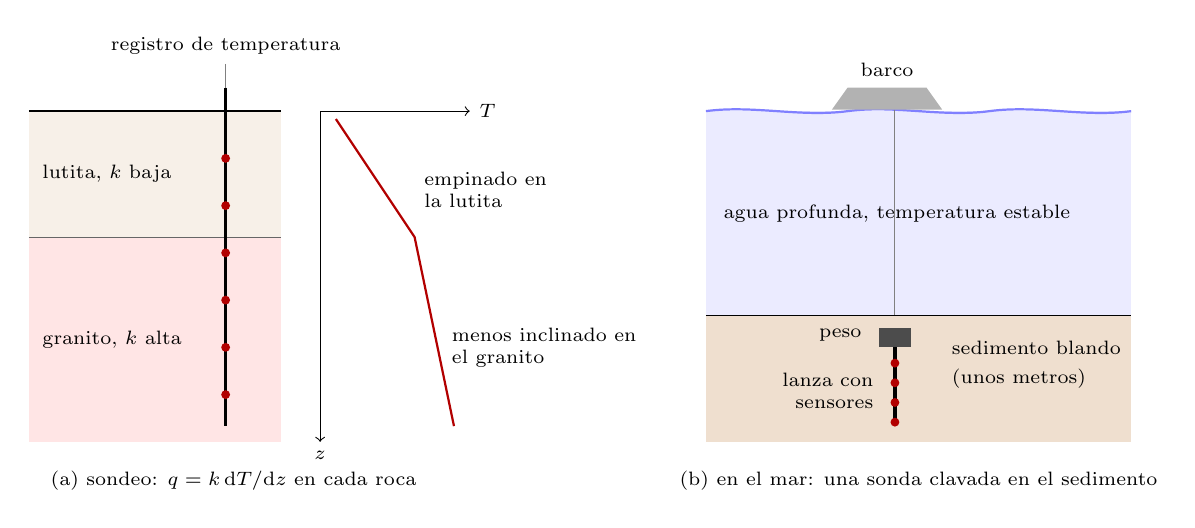
\begin{tikzpicture}[font=\scriptsize, x=1cm, y=1cm]
% --- left: borehole on land ---
\fill[brown!12] (0,0) rectangle (3.2,-1.6);
\fill[red!10] (0,-1.6) rectangle (3.2,-4.2);
\draw[thick] (0,0) -- (3.2,0);
\node[anchor=west] at (0.05,-0.8) {lutita, $k$ baja};
\node[anchor=west] at (0.05,-2.9) {granito, $k$ alta};
\draw[black!60] (0,-1.6) -- (3.2,-1.6);
\draw[very thick] (2.5,0.3) -- (2.5,-4.0);
\draw[gray] (2.5,0.6) -- (2.5,0.3);
\foreach \y in {-0.6,-1.2,-1.8,-2.4,-3.0,-3.6} {\fill[red!70!black] (2.5,\y) circle (1.6pt);}
\node[anchor=south] at (2.5,0.6) {registro de temperatura};
% inset T(z)
\draw[->] (3.7,0) -- (5.6,0) node[right] {$T$};
\draw[->] (3.7,0) -- (3.7,-4.2) node[below] {$z$};
\draw[thick, red!70!black] (3.9,-0.1) -- (4.9,-1.6) -- (5.4,-4.0);
\node[anchor=west, align=left] at (4.9,-1.0) {empinado en\\la lutita};
\node[anchor=west, align=left] at (5.25,-3.0) {menos inclinado en\\el granito};
\node[anchor=north] at (2.6,-4.45) {(a) sondeo: $q = k\,\mathrm dT/\mathrm dz$ en cada roca};
% --- right: probe at sea ---
\begin{scope}[xshift=8.6cm]
\fill[blue!8] (0,0) rectangle (5.4,-2.6);
\draw[blue!50, thick] (0,0) .. controls (0.6,0.08) and (1.2,-0.08) .. (1.8,0)
  .. controls (2.4,0.08) and (3.0,-0.08) .. (3.6,0) .. controls (4.2,0.08) and (4.8,-0.08) .. (5.4,0);
\fill[gray!60] (1.6,0.02) -- (3.0,0.02) -- (2.8,0.3) -- (1.8,0.3) -- cycle;
\node[anchor=south] at (2.3,0.32) {barco};
\draw[gray] (2.4,0.02) -- (2.4,-2.75);
\fill[brown!25] (0,-2.6) rectangle (5.4,-4.2);
\draw (0,-2.6) -- (5.4,-2.6);
\node[anchor=west] at (3.0,-3.0) {sedimento blando};
\node[anchor=west] at (3.0,-3.4) {(unos metros)};
\fill[black!70] (2.2,-2.75) rectangle (2.6,-3.0);
\draw[very thick] (2.4,-3.0) -- (2.4,-4.0);
\foreach \y in {-3.2,-3.45,-3.7,-3.95} {\fill[red!70!black] (2.4,\y) circle (1.6pt);}
\node[anchor=east, align=right] at (2.1,-2.85) {peso};
\node[anchor=east, align=right] at (2.25,-3.55) {lanza con\\sensores};
\node[anchor=west] at (0.1,-1.3) {agua profunda, temperatura estable};
\node[anchor=north] at (2.7,-4.45) {(b) en el mar: una sonda clavada en el sedimento};
\end{scope}
\end{tikzpicture}

\par\smallskip{\small Medición del \omterm{def:b1:heat-budget:heat-flow}{flujo de calor} (esquema, no a escala). (a) En tierra, la temperatura se registra a lo
largo de un sondeo una vez que ha vuelto al equilibrio, y la conductividad de cada roca se mide en testigos: el gradiente es
más empinado donde la conductividad es menor, y el \omterm{def:b1:heat-budget:heat-flow}{flujo de calor}, su producto, es el mismo. (b) En el mar, una lanza con
sensores se clava unos metros en el sedimento del fondo oceánico.}
\label{fig:b1:heat-budget:measure}
\end{omfigure}

\begin{inthefield}[Flujo de calor en el mar]
\begin{minipage}[t]{0.55\linewidth}\vspace{0pt}
En un buque de investigación, la sonda de \omterm{def:b1:heat-budget:heat-flow}{flujo de calor} es una lanza pesada suspendida de la grúa de popa. Se baja con el cable
del barco hasta justo encima del fondo marino, y luego se suelta: el peso la clava en el sedimento, y la tripulación espera en
cubierta a que los sensores se estabilicen a la temperatura del fango, después la saca y se desplaza a la siguiente estación, a poca
distancia. Una línea de estas estaciones a través del flanco de una dorsal da la disminución del \omterm{def:b1:heat-budget:heat-flow}{flujo de calor} con la edad del fondo,
y la dispersión entre estaciones vecinas muestra dónde circula agua por la \omterm{def:b1:layered-earth:layers}{corteza} subyacente.
\end{minipage}\hfill
\begin{minipage}[t]{0.42\linewidth}\vspace{0pt}
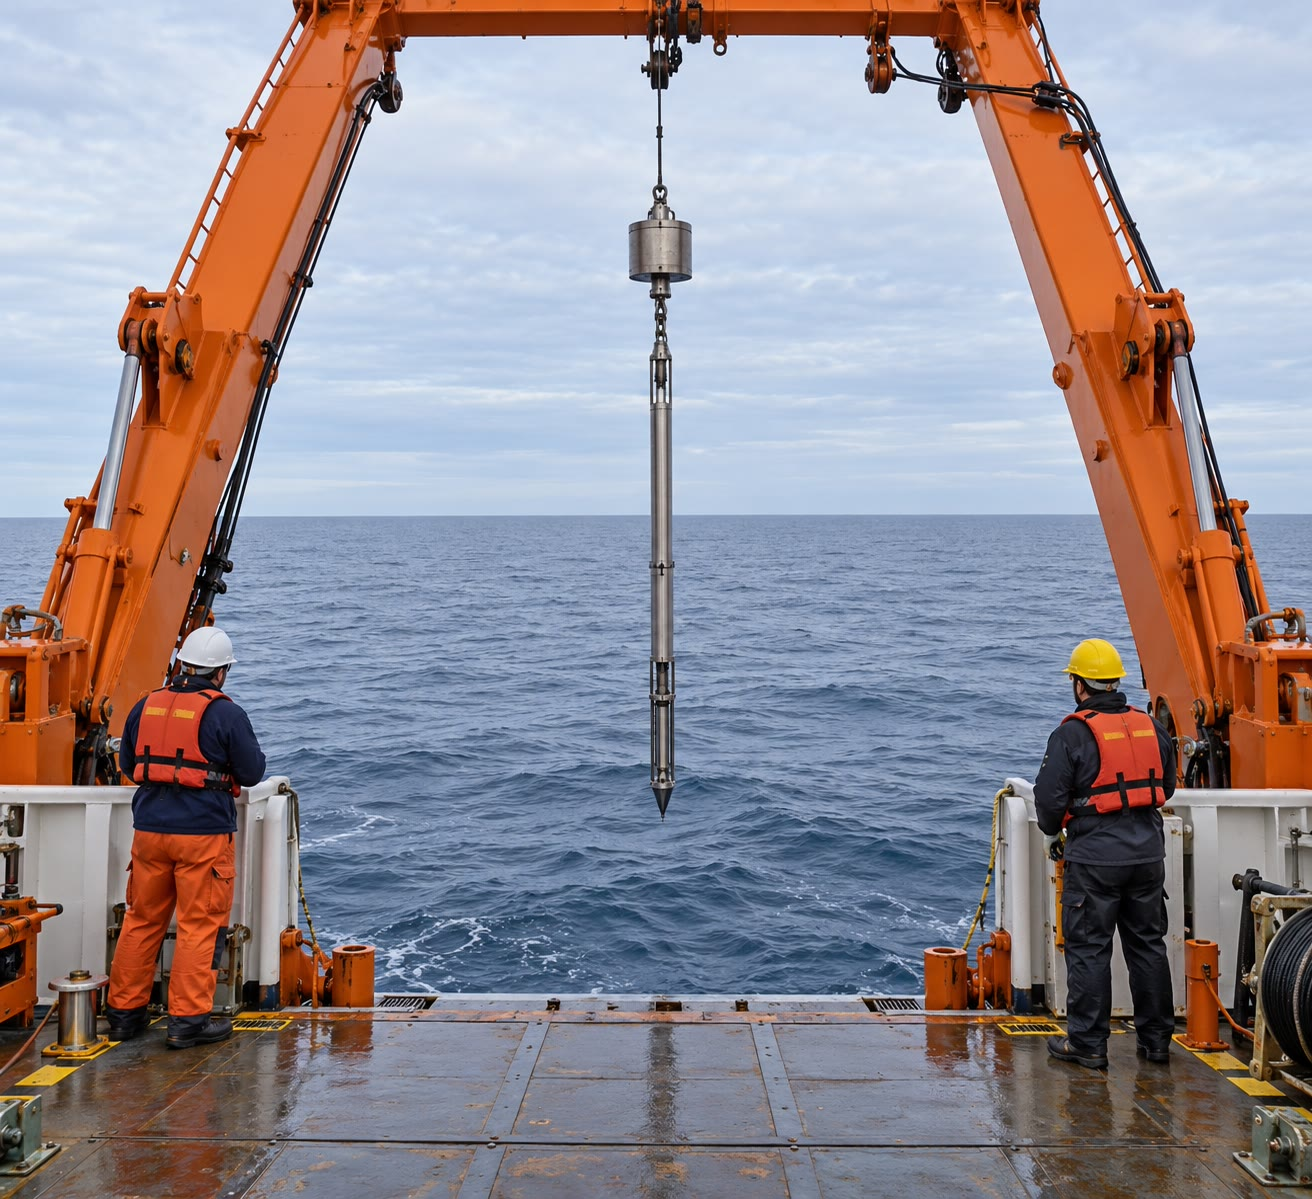
\includegraphics[width=\linewidth]{images/book3/ai/b1-heatflow-probe.jpg}

{\scriptsize Una sonda de \omterm{def:b1:heat-budget:heat-flow}{flujo de calor} colgada de la grúa de popa de un buque de investigación (ilustración generada por IA).}
\end{minipage}
\end{inthefield}

\section{El geotermo conductivo estacionario}

\begin{definition}[Geotermo]\label{def:b1:heat-budget:geotherm}
El \emph{geotermo}\index{geotermo} bajo un punto de la superficie es la temperatura en función de la profundidad allí, $T(z)$.
Es un geotermo conductivo estacionario cuando no cambia con el tiempo y el calor se transporta a lo largo de él solo por conducción.
\end{definition}

Dentro de la \omterm{def:b1:layered-earth:lithosphere}{litosfera}, lejos de los volcanes activos y de la circulación de agua, el calor se transporta por conducción, y a escala
de millones de años el \omterm{def:b1:heat-budget:geotherm}{geotermo} es estacionario. Su forma se deduce entonces de un balance de energía.

\begin{theorem}[Conducción estacionaria con producción de calor]\label{thm:b1:heat-budget:balance}
A lo largo de un \omterm{def:b1:heat-budget:geotherm}{geotermo} conductivo estacionario, en un medio de conductividad uniforme $k$ con producción de calor $A(z)$ y sin
flujo horizontal de calor,
\[
  \frac{\mathrm dq}{\mathrm dz} = -A(z), \qquad\text{es decir}\qquad
  k\,\frac{\mathrm d^2T}{\mathrm dz^2} = -A(z).
\]
\end{theorem}

\begin{proof}
Consideremos una losa horizontal de área $S$ entre las profundidades $z$ y $z +
\mathrm dz$. El calor entra por su base a razón de
$q(z + \mathrm dz)\,S$, sale por su techo a razón de $q(z)\,S$, y se produce en su interior a razón de $A(z)\,S\,\mathrm dz$. En un
régimen estacionario no se almacena calor, así que $q(z)\,S = q(z + \mathrm dz)\,S + A(z)\,S\,\mathrm dz$, lo que da
$\mathrm dq/\mathrm dz = -A$. Por la ley de Fourier $q = k\,\mathrm dT/\mathrm dz$, y con $k$ uniforme, $k\,T'' = -A$.
\end{proof}

Leído desde la superficie hacia abajo, el \omterm{def:b1:heat-budget:heat-flow}{flujo de calor} disminuye con la profundidad en el calor producido sobre cada nivel: lo que
atraviesa la superficie es el calor que viene de abajo más todo el calor producido por el camino. Dos distribuciones de $A$ dan
soluciones cerradas.

\begin{proposition}[Una capa radiogénica uniforme]\label{prop:b1:heat-budget:uniform}
Sea la producción de calor $A$ desde la superficie hasta la profundidad $h$ y cero debajo, la superficie a la temperatura $T_0$, y
el \omterm{def:b1:heat-budget:heat-flow}{flujo de calor} en la superficie $q_0$.
Entonces, para $0 \le z \le h$
\[
  q(z) = q_0 - A z, \qquad T(z) = T_0 + \frac{q_0 z}{k} - \frac{A z^2}{2k},
\]
y debajo de $h$ el \omterm{def:b1:heat-budget:heat-flow}{flujo de calor} es uniforme, $q_m = q_0 - A h$, y el \omterm{def:b1:heat-budget:geotherm}{geotermo} una recta de pendiente $q_m/k$.
\end{proposition}

\begin{proof}
Integrando $\mathrm dq/\mathrm dz = -A$ desde $0$ con $q(0) = q_0$: $q = q_0 -
Az$. Entonces $\mathrm dT/\mathrm dz = (q_0 - Az)/k$;
integrando con $T(0) = T_0$ se obtiene la parábola. Debajo de $h$, $\mathrm dq/\mathrm dz = 0$ y $q$ conserva su valor en $h$.
\end{proof}

\begin{theorem}[Producción de calor exponencial y relación lineal del flujo de calor]\label{thm:b1:heat-budget:exponential}
Sea la producción de calor que disminuye con la profundidad como $A(z) = A_0 e^{-z/D}$, el \omterm{def:b1:heat-budget:heat-flow}{flujo de calor} tiende a $q_m$ a gran
profundidad, y la superficie está a $T_0$. Entonces
\[
  q(z) = q_m + A_0 D\,e^{-z/D}, \qquad
  T(z) = T_0 + \frac{q_m z}{k} + \frac{A_0 D^2}{k}\bigl(1 - e^{-z/D}\bigr),
\]
y el \omterm{def:b1:heat-budget:heat-flow}{flujo de calor} en la superficie es
\[
  q_0 = q_m + A_0 D .
\]
\end{theorem}

\begin{proof}
Por \cref{thm:b1:heat-budget:balance}, $\mathrm dq/\mathrm dz =
-A_0e^{-z/D}$, así que $q(z) = A_0 D e^{-z/D} + C$; cuando $z \to \infty$,
$q \to C$, luego $C = q_m$. En $z = 0$, $q_0 = q_m + A_0 D$. Entonces $\mathrm dT/\mathrm dz =
q/k = q_m/k + (A_0D/k)\,e^{-z/D}$, e
integrando desde $0$ con $T(0) = T_0$, $T = T_0 + q_m z/k + (A_0 D^2/k)(1 - e^{-z/D})$.
\end{proof}

La última línea es una predicción que puede contrastarse en la superficie. Los plutones graníticos de una región comparten el mismo
flujo profundo $q_m$ y, si solo difieren en lo ricos que son en uranio, torio y potasio, la misma escala $D$; entonces el \omterm{def:b1:heat-budget:heat-flow}{flujo de calor}
medido sobre cada plutón debe ser una función lineal de la producción de calor medida en sus rocas, con pendiente $D$, una longitud,
y ordenada en el origen $q_m$, el flujo reducido, que procede de abajo y no del radiogénico.
Francis Birch observó por primera vez una recta así, publicada en 1968, y el mismo año se definieron tres provincias por sus rectas:
\begin{center}
\small
% ledger: roy:provinces, roy:linear-relation
\begin{tabular}{lcc}
\hline
provincia & ordenada en el origen $q_m$ (\unit{mW.m^{-2}}) & pendiente $D$ (\unit{km}) \\
\hline
Estados Unidos orientales & 33 & 7.5 \\
provincia de Basin and Range & 59 & 9.4 \\
Sierra Nevada & 17 & 10 \\
\hline
\end{tabular}
\end{center}
Las ordenadas en el origen, publicadas como 0.8, 1.4 y $0.4\times\qty{e-6}{cal.cm^{-2}.s^{-1}}$, se convierten con
$\qty{1}{\micro cal.cm^{-2}.s^{-1}} = \qty{41.84}{mW.m^{-2}}$ (\cref{exo:b1:heat-budget:4}). Las pendientes varían poco, de 7 a
\qty{10}{km}; el \omterm{def:b1:heat-budget:heat-flow}{flujo de calor} reducido varía mucho, y sus mapas muestran dónde el \omterm{def:b1:layered-earth:layers}{manto} de debajo está caliente, como bajo la
\omterm{def:b1:layered-earth:layers}{corteza} adelgazada de Basin and Range. La capa uniforme de \cref{prop:b1:heat-budget:uniform} da también una recta, de pendiente
$h$: ambos modelos ajustan los datos, pero solo el exponencial sigue siendo una recta de la misma pendiente cuando los plutones se
erosionan hasta profundidades distintas (\cref{exo:b1:heat-budget:10}), por lo que se prefiere.

\begin{omfigure}
\begin{tikzpicture}
\begin{axis}[omdepth, width=0.82\linewidth, height=8.6cm, xmin=0, xmax=1800, ymin=0, ymax=250, axis x line=top, axis y line=left, axis line style={-}, clip=true,
  xlabel={temperatura (\unit{\degreeCelsius})}, ylabel={profundidad (km)},
  tick label style={font=\scriptsize}, label style={font=\small},
  legend style={font=\scriptsize, at={(0.02,0.02)}, anchor=south west, draw=none, fill=white, fill opacity=0.85, text opacity=1},
  legend cell align=left]
\addplot[very thick, black!45] table[x=T, y=depth] {figdata/out/bachelor-1-geotherms-adiabat.dat};
\addlegendentry{adiabática del manto}
\addplot[very thick, red!75!black] table[x=T45, y=depth] {figdata/out/bachelor-1-geotherms-continental.dat};
\addlegendentry{$q_0 = \qty{70}{mW.m^{-2}}$}
\addplot[very thick, orange!80!black] table[x=T30, y=depth] {figdata/out/bachelor-1-geotherms-continental.dat};
\addlegendentry{$q_0 = \qty{55}{mW.m^{-2}}$}
\addplot[very thick, green!45!black] table[x=T15, y=depth] {figdata/out/bachelor-1-geotherms-continental.dat};
\addlegendentry{$q_0 = \qty{40}{mW.m^{-2}}$}
\addplot[thick, blue!70!black, densely dashdotted] table[x=T, y=depth] {figdata/out/bachelor-1-geotherms-oceanic.dat};
\addlegendentry{fondo oceánico de \qty{60}{Myr}}
\addplot[thin, dashed, red!75!black, forget plot] table[x=Tc45, y=depth] {figdata/out/bachelor-1-geotherms-continental.dat};
\addplot[thin, dashed, orange!80!black, forget plot] table[x=Tc30, y=depth] {figdata/out/bachelor-1-geotherms-continental.dat};
\addplot[thin, dashed, green!45!black, forget plot] table[x=Tc15, y=depth] {figdata/out/bachelor-1-geotherms-continental.dat};
\draw[densely dotted, black!60] (axis cs:0,35) -- (axis cs:1800,35);
\node[font=\scriptsize, anchor=south east] at (axis cs:1790,35) {Moho, \qty{35}{km}};
\fill (axis cs:1384.0,70.8) circle (1.6pt);
\fill (axis cs:1403.2,107.8) circle (1.6pt);
\fill (axis cs:1459.7,224.9) circle (1.6pt);
\node[font=\scriptsize, anchor=west] at (axis cs:1420,66) {\qty{71}{km}};
\node[font=\scriptsize, anchor=west] at (axis cs:1440,104) {\qty{108}{km}};
\node[font=\scriptsize, anchor=west] at (axis cs:1495,222) {\qty{225}{km}};
\end{axis}
\end{tikzpicture}

\par\smallskip{\small \omterm{def:b1:heat-budget:geotherm}{Geotermos} conductivos estacionarios de un continente con producción de calor $A_0 = \qty{2.5}{\micro W.m^{-3}}$
que disminuye sobre $D = \qty{10}{km}$, $k = \qty{2.5}{W.m^{-1}.K^{-1}}$, para tres \omterm{def:b1:heat-budget:heat-flow}{flujos de calor} en superficie (flujos
reducidos de 15, 30 y \qty{45}{mW.m^{-2}}). Cada uno sigue su curva conductiva (discontinua más allá) hasta la \omterm{def:b1:heat-budget:adiabat}{adiabática del manto},
a la que llega en el punto: la base de la \omterm{def:b1:heat-budget:boundary-layer}{litosfera térmica}. El \omterm{def:b1:heat-budget:geotherm}{geotermo} del fondo oceánico es el de un semiespacio enfriado durante
\qty{60}{Myr}. La conductividad uniforme es una simplificación.}
\label{fig:b1:heat-budget:geotherms}
\end{omfigure}

\begin{method}[La temperatura a profundidad bajo un plutón]\label{met:b1:heat-budget:moho}
\begin{enumerate}
  \item Mídase el \omterm{def:b1:heat-budget:heat-flow}{flujo de calor} en superficie $q_0$ sobre el plutón (método del sondeo) y su producción de calor $A_0$ a partir de
        sus contenidos en U, Th y K.
  \item A partir de la recta de la provincia, o con un valor de $D$ de unos \qty{10}{km}, calcúlese $q_m = q_0 - A_0 D$.
  \item Aplíquese \cref{thm:b1:heat-budget:exponential}. Por debajo de unas pocas veces $D$, $e^{-z/D}$ es despreciable y el
        \omterm{def:b1:heat-budget:geotherm}{geotermo} es la recta $T_0 + A_0D^2/k + q_m z/k$: la capa radiogénica ha elevado toda temperatura profunda en $A_0D^2/k$.
\end{enumerate}
\end{method}

En la figura, la temperatura en el \omterm{def:b1:layered-earth:discontinuity}{Moho} va de unos \qty{320}{\degreeCelsius} para el flujo más bajo a más de \qty{700}{\degreeCelsius}
para el más alto: el \omterm{def:b1:heat-budget:heat-flow}{flujo de calor} en superficie lleva una lectura directa de la temperatura de la \omterm{def:b1:layered-earth:layers}{corteza} profunda, que gobierna
su resistencia (\cref{ch:b1:stress-strain-rheology}).

\section{Conducción frente a convección}

La conducción es lenta. Lo lenta que es se deduce de la ecuación del calor, que los libros de física deducen de la ley de Fourier y
del balance de \cref{thm:b1:heat-budget:balance} con el almacenamiento añadido: en una dimensión, sin producción de calor,
$\partial T/\partial t = \kappa\,\partial^2 T/\partial z^2$.

\begin{proposition}[La escala de tiempo conductiva]\label{prop:b1:heat-budget:timescale}
Una variación de temperatura impuesta en la frontera de un cuerpo conductor se extiende una distancia $L$ en un tiempo del orden de
\[
  \tau = \frac{L^2}{\kappa} .
\]
\end{proposition}

\begin{proof}
Escríbase $z = L z^*$, $t = \tau t^*$, con $z^*$ y $t^*$ adimensionales. La ecuación del calor queda $\partial T/\partial t^* = (\kappa\tau/L^2)\,\partial^2
T/\partial z^{*2}$. Sus soluciones varían en la escala $z^* \sim 1$ cuando $t^* \sim 1$
solo si el coeficiente es de orden uno, es decir, si $\tau \sim L^2/\kappa$.
\end{proof}

Las rocas tienen $\kappa \approx \qty{e-6}{m^2.s^{-1}}$. El ciclo térmico diario llega a unas decenas de centímetros
bajo el suelo, el anual a unos metros, y el calentamiento desde la última glaciación a un kilómetro
más o menos. En una \omterm{def:b1:layered-earth:lithosphere}{litosfera} de \qty{100}{km} de espesor, $\tau = \qty{e16}{s}$, unos \qty{300}{Myr}. A través
del \omterm{def:b1:layered-earth:layers}{manto}, de \qty{2900}{km} de espesor, $\tau = \qty{8.4e18}{s}$, o \qty{270}{Gyr}: sesenta veces la edad
de la Tierra, \qty{4.54}{Gyr}. % ledger: england:kelvin, usgs:age-earth
La conducción sola no podría haber llevado el calor del \omterm{def:b1:layered-earth:layers}{manto} profundo a ningún punto cercano a la superficie.
El \omterm{def:b1:layered-earth:layers}{manto} convecta, y en su interior el calor lo transporta el movimiento de la propia roca, a las velocidades
de las placas, centímetros por año. % ledger: usgs:san-andreas

\begin{definition}[Adiabática del manto]\label{def:b1:heat-budget:adiabat}
La \emph{adiabática del manto}\index{adiabática del manto} es el \omterm{def:b1:heat-budget:geotherm}{geotermo} del interior bien mezclado del \omterm{def:b1:layered-earth:layers}{manto} en convección: la
temperatura que toma la roca del \omterm{def:b1:layered-earth:layers}{manto} al subir o bajar con la rapidez suficiente para no intercambiar calor con su entorno,
enfriándose por expansión al subir y calentándose por compresión al bajar.
\end{definition}

La termodinámica da su gradiente, $\mathrm dT/\mathrm dz = \alpha g T/c_p$, con $\alpha$ la expansividad térmica y $c_p$
el calor específico (física, admitido aquí). Es pequeño. Una evaluación reciente de la física \omterm{def:b1:rock-forming-minerals:mineral}{mineral} da
\qty{0.54}{K.km^{-1}} a \qty{50}{km} de profundidad, que baja hasta \qty{0.36}{K.km^{-1}} a \qty{410}{km}, y luego de 0.41 a
\qty{0.23}{K.km^{-1}} en el \omterm{def:b1:layered-earth:layers}{manto} inferior, con \qty{1646}{K} a \qty{50}{km} y \qty{2587}{K} a \qty{2800}{km}.
% ledger: katsura:adiabat
Extrapolada a la superficie, la adiabática da la temperatura potencial del \omterm{def:b1:layered-earth:layers}{manto}, \qty{1619}{K} o unos \qty{1350}{\degreeCelsius}:
la temperatura que tendría el \omterm{def:b1:layered-earth:layers}{manto} si se subiera a la superficie sin intercambiar calor. La noción de temperatura potencial se
define, para la atmósfera y el océano, en \cref{ch:b1:fluid-envelopes-structure}. Una temperatura que aumenta solo \qty{0.5}{K}
por kilómetro, mientras el \omterm{def:b1:heat-budget:geotherm}{geotermo} conductivo cerca de la superficie sube \qty{25}{K}, es la firma de la convección.

\begin{history}[John Perry y la Tierra que se enfría]
En 1862--1863 William Thomson, después Lord Kelvin, calculó la edad de la Tierra a partir de su enfriamiento. La trató como un sólido que se había enfriado por conducción desde una temperatura uniforme de unos \qty{3900}{\degreeCelsius};
con el gradiente medio de su época, unos \qty{36}{K.km^{-1}}, que eligió a partir de las medidas de entonces, y una difusividad de
\qty{1.2e-6}{m^2.s^{-1}}, el tiempo necesario para alcanzar el gradiente actual fue de unos \qty{96}{Myr}, entre cotas de 24 y \qty{400}{Myr} (\cref{exo:b1:heat-budget:9}). Los geólogos lo juzgaron demasiado corto.
En 1895, un año antes del descubrimiento de la radiactividad, su antiguo ayudante John Perry señaló en cambio una suposición:
si el interior era en parte fluido y convectaba, transportaría el calor como si tuviera una conductividad enorme, y todo el interior,
no solo una cáscara exterior delgada, alimentaría el \omterm{def:b1:heat-budget:heat-flow}{flujo de calor} en superficie. Su argumento fue ignorado y olvidado;
la convección del \omterm{def:b1:layered-earth:layers}{manto}, establecida mucho después, le dio la razón: el \omterm{def:b1:layered-earth:layers}{manto} profundo se enfría por convección, y eso es
el \omterm{def:b1:heat-budget:secular-cooling}{enfriamiento secular} del balance. % ledger: england:kelvin, england:perry
\end{history}

\begin{proposition}[La Tierra bien agitada de Perry]\label{prop:b1:heat-budget:perry}
Sea una esfera de radio $R$ con un interior bien agitado a la temperatura uniforme $T_i(t)$, con capacidad calorífica $\rho c$ por
unidad de volumen, bajo una tapa conductora de espesor $L \ll R$ y conductividad $k$ cuya superficie está a
$\qty{0}{\degreeCelsius}$, y sin producción de calor. Entonces
\[
  T_i(t) = T_i(0)\,e^{-t/\tau_P}, \qquad \tau_P = \frac{RL}{3\kappa},
\]
y el \omterm{def:b1:heat-budget:heat-flow}{flujo de calor} en superficie $kT_i/L$ decae con la misma constante de tiempo.
\end{proposition}

\begin{proof}
Como la tapa es delgada, está en estado estacionario y transporta el \omterm{def:b1:heat-budget:heat-flow}{flujo de calor}
$q = kT_i/L$. El interior pierde su calor a través del área $4\pi R^2$:
$\tfrac43\pi R^3\rho c\,\mathrm dT_i/\mathrm dt = -4\pi R^2 kT_i/L$, que es
$\mathrm dT_i/\mathrm dt = -3\kappa T_i/(RL)$ con $\kappa = k/(\rho c)$, cuya
solución es la exponencial de $\tau_P = RL/(3\kappa)$.
\end{proof}

Para $R = \qty{6400}{km}$, $L = \qty{100}{km}$ y $\kappa =
\qty{e-6}{m^2.s^{-1}}$, $\tau_P = \qty{6.8}{Gyr}$: una Tierra que
convecta mantiene un \omterm{def:b1:heat-budget:heat-flow}{flujo de calor} alto durante miles de millones de años, donde la Tierra conductora de Kelvin lo perdió en
decenas de millones (\cref{exo:b1:heat-budget:11}).

\section{La litosfera como capa límite térmica}\label{sec:b1:heat-budget:boundary-layer}

\begin{definition}[Capa límite térmica, litosfera térmica]\label{def:b1:heat-budget:boundary-layer}
En un fluido que convecta, una \emph{capa límite térmica}\index{capa límite térmica} es una capa a lo largo de un contorno en la que
el calor pasa por conducción y la temperatura cambia del valor del contorno al del interior bien mezclado. La \emph{litosfera
térmica}\index{litosfera térmica} es la capa límite térmica superior del \omterm{def:b1:layered-earth:layers}{manto}: la cáscara exterior de la Tierra, desde la superficie
hasta la profundidad a la que el \omterm{def:b1:heat-budget:geotherm}{geotermo} conductivo se encuentra con la \omterm{def:b1:heat-budget:adiabat}{adiabática del manto}.
\end{definition}

Las placas son la parte fría superior de la convección del \omterm{def:b1:layered-earth:layers}{manto}, su capa límite superior. Su base, donde el \omterm{def:b1:heat-budget:geotherm}{geotermo} conductivo
empinado se curva hacia la adiabática suave, está a \qtyrange{70}{230}{km} en la figura de los \omterm{def:b1:heat-budget:geotherm}{geotermos} para \omterm{def:b1:heat-budget:heat-flow}{flujos de calor}
continentales de 70 a \qty{40}{mW.m^{-2}}, en el rango medido por sismología (\cref{ch:b1:layered-earth}): la \omterm{def:b1:layered-earth:lithosphere}{litosfera} definida por
su resistencia y la definida por su temperatura son aproximadamente la misma cáscara, porque la resistencia depende de la
temperatura. En el fondo del \omterm{def:b1:layered-earth:layers}{manto}, la capa D$''$ es la capa límite inferior, calentada desde abajo por el núcleo.

Bajo los océanos, la capa límite nace en la dorsal, donde el \omterm{def:b1:layered-earth:layers}{manto} caliente sube a la superficie, y se engrosa a medida que la placa
se aleja y se enfría. El enfriamiento de un semiespacio desde una temperatura uniforme, resuelto por Fourier y usado por Kelvin para
la Tierra entera, lo describe bien (\cref{ch:b1:rifts-ridges-margins} y el libro de tercer año universitario lo deducen): las
isotermas se hunden como la raíz cuadrada de la edad del fondo (figura de abajo), y el \omterm{def:b1:heat-budget:heat-flow}{flujo de calor} disminuye como
\[
  q(t) = \frac{C}{\sqrt t}, \qquad C \approx \qty{490}{mW.m^{-2}.Myr^{1/2}},
\]
el valor empleado en el balance global. % ledger: dd10:young-ocean
A \qty{100}{Myr} el semiespacio se ha enfriado hasta unos \qty{130}{km} (\cref{exo:b1:heat-budget:12}). La placa real deja de
engrosarse antes: las ondas sísmicas que cruzan el Pacífico se ajustan mejor con una placa enfriada que tiende a un espesor de
\qtyrange{85}{95}{km}, el aplanamiento del fondo oceánico antiguo que se vuelve a encontrar en \cref{ch:b1:rifts-ridges-margins}.
% ledger: fischer:lithosphere

El balance térmico, el \omterm{def:b1:heat-budget:heat-flow}{flujo de calor} y la estructura térmica de las placas se reúnen en los capítulos siguientes: la placa enfriada
se hunde (\cref{ch:b1:rifts-ridges-margins}), y la \omterm{def:b1:layered-earth:lithosphere}{litosfera} fría que se hunde en las zonas de subducción es la corriente
descendente de la convección a la que pertenece.

\begin{omfigure}
\begin{tikzpicture}
\begin{axis}[width=0.86\linewidth, height=5.6cm, xmin=0, xmax=100, ymin=0, ymax=170,
  y dir=reverse, axis x line=top, axis y line=left, axis line style={-}, clip=false,
  xlabel={edad del fondo oceánico (Myr), que crece con la distancia a la dorsal},
  ylabel={profundidad (km)}, tick label style={font=\scriptsize}, label style={font=\small}]
\addplot[fill=blue!12, draw=none] table[x=age, y=z1200] {figdata/out/bachelor-1-geotherms-isotherms.dat} \closedcycle;
\addplot[thick, blue!30!black] table[x=age, y=z400] {figdata/out/bachelor-1-geotherms-isotherms.dat};
\addplot[thick, blue!50!red] table[x=age, y=z800] {figdata/out/bachelor-1-geotherms-isotherms.dat};
\addplot[very thick, red!75!black] table[x=age, y=z1200] {figdata/out/bachelor-1-geotherms-isotherms.dat};
\node[font=\scriptsize, anchor=south, fill=blue!12, inner sep=1pt] at (axis cs:80,24) {\qty{400}{\degreeCelsius}};
\node[font=\scriptsize, anchor=south, fill=blue!12, inner sep=1pt] at (axis cs:80,55) {\qty{800}{\degreeCelsius}};
\node[font=\scriptsize, anchor=south, fill=blue!12, inner sep=1pt] at (axis cs:80,108) {\qty{1200}{\degreeCelsius}};
\node[font=\small] at (axis cs:60,72) {litosfera térmica};
\node[font=\small] at (axis cs:55,150) {manto en convección, unos \qty{1350}{\degreeCelsius}};
\draw[->, thick, red!60!black] (axis cs:3,165) -- (axis cs:3,125);
\node[font=\scriptsize, anchor=west, red!60!black] at (axis cs:4,140) {ascenso bajo la dorsal};
\draw[->, thick, black!60] (axis cs:30,5) -- (axis cs:70,5);
\node[font=\scriptsize, anchor=west] at (axis cs:70,5) {movimiento de la placa};
\end{axis}
\end{tikzpicture}

\par\smallskip{\small Isotermas en una placa oceánica que se enfría: un semiespacio inicialmente a \qty{1350}{\degreeCelsius},
enfriado desde su superficie, con
$\kappa = \qty{e-6}{m^2.s^{-1}}$. Cada isoterma se hunde como la raíz cuadrada de la edad; la
capa sombreada sobre la isoterma de \qty{1200}{\degreeCelsius} es la \omterm{def:b1:heat-budget:boundary-layer}{litosfera térmica}. Las flechas son esquemáticas.}
\label{fig:b1:heat-budget:isotherms}
\end{omfigure}

\section{Ejercicios}

\begin{exercise}[$\star$]\label{exo:b1:heat-budget:1}
Un sondeo en granito de conductividad \qty{2.5}{W.m^{-1}.K^{-1}} muestra un gradiente estacionario de \qty{22}{K.km^{-1}}.
Calcúlese el \omterm{def:b1:heat-budget:heat-flow}{flujo de calor} y la potencia que atraviesa un kilómetro cuadrado de superficie en ese punto.
% ledger: delaney:conductivity
\end{exercise}

\begin{exercise}[$\star$]\label{exo:b1:heat-budget:2}
A partir de las áreas y los \omterm{def:b1:heat-budget:heat-flow}{flujos de calor} medios de los continentes (\qty{2.073e14}{m^2}, \qty{70.9}{mW.m^{-2}}) y de los océanos
(\qty{3.028e14}{m^2}, \qty{105.4}{mW.m^{-2}}), calcúlese la pérdida de calor de cada uno, la total y el \omterm{def:b1:heat-budget:heat-flow}{flujo de calor} medio sobre la
superficie de la Tierra (\qty{5.101e14}{m^2}). ¿Qué fracción de los \qty{173000}{TW} que recibe del Sol representa?
% ledger: dd10:split, nasa:solar-mean
\end{exercise}

\begin{exercise}[$\star$]\label{exo:b1:heat-budget:3}
A partir de la tabla de los cuatro isótopos, calcúlese el calor liberado por kilogramo de uranio natural
(\qty{99.274}{\percent} \ce{^{238}U} y \qty{0.720}{\percent} \ce{^{235}U} de los átomos; sus masas difieren en unos
\qty{1}{\percent}, así que tómense estas como fracciones másicas) y por kilogramo de potasio natural, cuyo \ce{^{40}K} constituye
el \qty{0.0117}{\percent} de los átomos (tómese la masa de un átomo de \ce{^{40}K} como $39.96/39.10$ veces la masa media de un átomo de potasio).
% ledger: dye:isotope-heat, iaea:isotopes
\end{exercise}

\begin{exercise}[$\star$]\label{exo:b1:heat-budget:4}
Conviértanse las ordenadas en el origen de las tres provincias, 0.8, 1.4 y $0.4\times\qty{e-6}{cal.cm^{-2}.s^{-1}}$, a \unit{mW.m^{-2}}
($\qty{1}{cal} = \qty{4.184}{J}$). Prevéase el \omterm{def:b1:heat-budget:heat-flow}{flujo de calor} en superficie sobre un granito de producción de calor
\qty{3.0}{\micro W.m^{-3}} en cada provincia.
% ledger: roy:provinces
\end{exercise}

\begin{exercise}[$\star\star$]\label{exo:b1:heat-budget:5}
Una \omterm{def:b1:layered-earth:layers}{corteza} tiene una producción de calor uniforme de \qty{2.0}{\micro W.m^{-3}} en sus \qty{10}{km} superiores y ninguna por debajo,
una conductividad de \qty{2.5}{W.m^{-1}.K^{-1}}, un \omterm{def:b1:heat-budget:heat-flow}{flujo de calor} en superficie de \qty{60}{mW.m^{-2}} y una temperatura en superficie
de \qty{10}{\degreeCelsius}. Calcúlense la temperatura a \qty{10}{km}, el \omterm{def:b1:heat-budget:heat-flow}{flujo de calor} bajo la capa radiogénica y la temperatura
en el \omterm{def:b1:layered-earth:discontinuity}{Moho}, a \qty{35}{km} de profundidad.
\end{exercise}

\begin{exercise}[$\star\star$]\label{exo:b1:heat-budget:6}
Un sondeo atraviesa \qty{300}{m} de lutita ($k = \qty{1.5}{W.m^{-1}.K^{-1}}$), y luego granito ($k = \qty{3.0}{W.m^{-1}.K^{-1}}$).
Las \omterm{def:b1:comparative-planetology:equilibrium-temperature}{temperaturas de equilibrio} son \qty{12.0}{\degreeCelsius} en superficie, \qty{24.0}{\degreeCelsius} a \qty{300}{m} y
\qty{34.0}{\degreeCelsius} a \qty{800}{m}. Calcúlense el gradiente y el \omterm{def:b1:heat-budget:heat-flow}{flujo de calor} en cada roca, la resistencia térmica a
\qty{300}{m} y a \qty{800}{m}, y la pendiente del diagrama de Bullard. ¿Es constante el \omterm{def:b1:heat-budget:heat-flow}{flujo de calor}?
\end{exercise}

\begin{exercise}[$\star\star$]\label{exo:b1:heat-budget:7}
Con $\kappa = \qty{e-6}{m^2.s^{-1}}$, calcúlese la escala de tiempo conductiva para $L = \qty{1}{m}$, \qty{10}{m},
\qty{100}{km} y \qty{2900}{km}, cada una en una unidad adecuada. ¿Qué ciclos de temperatura en superficie se siguen sintiendo
\qty{10}{m} bajo el suelo? Compárese el último tiempo con la edad de la Tierra.
% ledger: england:kelvin, usgs:age-earth
\end{exercise}

\begin{exercise}[$\star\star$]\label{exo:b1:heat-budget:8}
La \omterm{def:b1:heat-budget:adiabat}{adiabática del manto} está a \qty{1646}{K} a \qty{50}{km} de profundidad, con un gradiente de \qty{0.54}{K.km^{-1}} allí, que
disminuye hasta \qty{0.36}{K.km^{-1}} a \qty{410}{km}. (a) Extrapólese hasta la superficie con el gradiente a \qty{50}{km}, y
dése la temperatura potencial en kelvin y en grados Celsius. (b) Estímese la temperatura a \qty{410}{km} con la media de los dos
gradientes, y compárese con los \qty{1799}{K} publicados justo encima de la discontinuidad.
% ledger: katsura:adiabat
\end{exercise}

\begin{exercise}[$\star\star$]\label{exo:b1:heat-budget:9}
Un semiespacio enfriado desde la temperatura uniforme $T_0$, con su superficie mantenida a
$\qty{0}{\degreeCelsius}$, tiene tras un tiempo $t$ el gradiente superficial $G =
T_0/\sqrt{\pi\kappa t}$ (admitido). (a) Exprésese $t$ en función de $G$. (b) Con los valores de Kelvin,
$T_0 = \qty{3900}{\degreeCelsius}$, $\kappa =
\qty{1.2e-6}{m^2.s^{-1}}$ y $G = 1/50$ de grado Fahrenheit por pie; calcúlese $G$ en \unit{K.km^{-1}} y la edad.
(c) Rehágase con $T_0 =
\qty{1300}{\degreeCelsius}$, $\kappa = \qty{e-6}{m^2.s^{-1}}$ y $G =
\qty{36}{K.km^{-1}}$.
% ledger: england:kelvin
\end{exercise}

\begin{exercise}[$\star\star\star$]\label{exo:b1:heat-budget:10}
Una provincia se erosiona: se retira un espesor $e$ de la parte superior de cada plutón, siendo inalterado el flujo profundo $q_m$.
(a) En el modelo exponencial, muéstrese que la nueva producción superficial de calor y el nuevo \omterm{def:b1:heat-budget:heat-flow}{flujo de calor}, $A_0'$ y $q_0'$,
siguen cumpliendo $q_0' = q_m + A_0'D$. (b) En el modelo de capa uniforme de espesor $h$, muéstrese que un plutón erosionado
en $e$ se sitúa en una recta de pendiente $h - e$. (c) Plutones de una misma provincia se erosionaron en cantidades distintas.
¿Qué modelo predice que siguen sobre una sola recta?
\end{exercise}

\begin{exercise}[$\star\star\star$]\label{exo:b1:heat-budget:11}
En el modelo de Perry (\cref{prop:b1:heat-budget:perry}) tómese $R = \qty{6400}{km}$,
$\kappa = \qty{e-6}{m^2.s^{-1}}$, $k = \qty{3}{W.m^{-1}.K^{-1}}$ y una temperatura interior inicial de \qty{1300}{\degreeCelsius}. (a) Calcúlese $\tau_P$ para tapas
de 50 y \qty{100}{km}. (b) Para la tapa de \qty{50}{km}, calcúlese el \omterm{def:b1:heat-budget:heat-flow}{flujo de calor} en superficie al principio y tras
\qty{2}{Gyr}. (c) El semiespacio conductor de Kelvin, con el mismo $k$ y $T_0$, tiene un \omterm{def:b1:heat-budget:heat-flow}{flujo de calor} en superficie
$kT_0/\sqrt{\pi\kappa t}$: calcúlese tras \qty{2}{Gyr} y compárese.
% ledger: england:kelvin, england:perry
\end{exercise}

\begin{exercise}[$\star\star\star$]\label{exo:b1:heat-budget:12}
El \omterm{def:b1:heat-budget:heat-flow}{flujo de calor} en superficie de un semiespacio que se enfría es $q = k\,\Delta T/\sqrt{\pi\kappa t}$
(\cref{exo:b1:heat-budget:9}). (a) Con $k = \qty{3}{W.m^{-1}.K^{-1}}$, $\kappa =
\qty{e-6}{m^2.s^{-1}}$ y $\Delta T = \qty{1336}{K}$ (desde la temperatura potencial hasta un fondo marino a unos
\qty{10}{\degreeCelsius}), calcúlese la constante $C$ de $q = C/\sqrt t$, con $t$ en millones de años, y compárese con los
\qty{490}{mW.m^{-2}.Myr^{1/2}} ajustados a los datos. (b) Con $C = 490$, dense el \omterm{def:b1:heat-budget:heat-flow}{flujo de calor} a 1, 10 y \qty{100}{Myr}. (c) La
isoterma de \qty{1200}{\degreeCelsius} de la figura de isotermas en enfriamiento se encuentra donde $z = 2\times1.163\sqrt{\kappa t}$;
calcúlese su profundidad a \qty{100}{Myr}.
% ledger: dd10:young-ocean, katsura:adiabat, fischer:lithosphere
\end{exercise}

\section{Problema: rocas calientes bajo los plutones}

\begin{problem}[{Problema de fin de semana --- flujo de calor y producción de calor de cinco plutones graníticos, la relación lineal y la temperatura de la corteza profunda}]
\label{pb:b1:heat-budget:1}
% values: calc/ch10.py (invented province; element heats from the chapter's table)
% ledger: dye:isotope-heat, iaea:isotopes, dd10:split, roy:provinces
Se han perforado cinco plutones graníticos de una misma provincia. En cada sondeo se registró la \omterm{def:b1:comparative-planetology:equilibrium-temperature}{temperatura de equilibrio} a
\qty{100}{m} y a \qty{500}{m}, y la conductividad del granito se midió en testigos; sus contenidos de uranio, torio y
potasio se analizaron en muestras de superficie. Los cinco granitos tienen una densidad de \qty{2650}{kg.m^{-3}}.
\begin{center}
\small
\begin{tabular}{cccccc}
\hline
plutón & $T$ a \qty{100}{m} (\unit{\degreeCelsius}) & $T$ a \qty{500}{m} (\unit{\degreeCelsius}) & $k$ (\unit{W.m^{-1}.K^{-1}}) & U, Th (ppm) & K (\unit{\percent}) \\
\hline
A & 13.1 & 19.2 & 2.9 & 2.0, 8 & 3.0 \\
B & 12.4 & 20.2 & 2.6 & 3.5, 14 & 3.5 \\
C & 13.6 & 21.4 & 3.1 & 5.0, 18 & 4.0 \\
D & 12.9 & 23.1 & 2.7 & 7.0, 25 & 4.2 \\
E & 14.2 & 25.5 & 3.0 & 10.0, 35 & 4.5 \\
\hline
\end{tabular}
\end{center}
Úsense los calores elementales $\qty{9.85e-5}{W.kg^{-1}}$ (U), $\qty{2.63e-5}{W.kg^{-1}}$
(Th) y $\qty{3.40e-9}{W.kg^{-1}}$ (K). Bajo los plutones, tómese
$k = \qty{2.5}{W.m^{-1}.K^{-1}}$ para toda la \omterm{def:b1:layered-earth:layers}{corteza} y una temperatura en superficie de
\qty{10}{\degreeCelsius}.

\medskip
\noindent\textbf{Parte I --- Flujo de calor.}
\begin{enumerate}
  \item Calcúlese el gradiente de temperatura en cada sondeo.
  \item ¿Por qué deben registrarse las temperaturas semanas o meses después de la perforación, y por qué se deja fuera
        la parte superior de \qty{100}{m}?
  \item Calcúlese el \omterm{def:b1:heat-budget:heat-flow}{flujo de calor} en cada plutón.
  \item Compárense con el \omterm{def:b1:heat-budget:heat-flow}{flujo de calor} continental medio, \qty{70.9}{mW.m^{-2}}.
  \item Los gradientes de B y de C son iguales. ¿Por qué no lo son sus \omterm{def:b1:heat-budget:heat-flow}{flujos de calor}?
  \item Los plutones están bajo colinas. ¿Elevaría o bajaría el relieve el gradiente medido bajo una cima?
        (Piénsese en la forma de las isotermas.)
\end{enumerate}

\noindent\textbf{Parte II --- Producción de calor y la recta.}
\begin{enumerate}[resume]
  \item Calcúlese la producción de calor debida al uranio en cada plutón.
  \item Lo mismo para el torio.
  \item Lo mismo para el potasio.
  \item Súmense para obtener $A_0$ en cada plutón. ¿Qué elemento contribuye
        menos?
  \item Represéntese $q_0$ frente a $A_0$. ¿Están los puntos cerca de una recta?
  \item Calcúlense las medias de $A_0$ y de $q_0$, y las sumas
        $\sum (A_0 - \bar A_0)^2$ y $\sum (A_0 - \bar A_0)(q_0 - \bar q_0)$.
  \item Dedúzcase la recta de mínimos cuadrados $q_0 = q_m + D A_0$: su pendiente $D$ (en
        \unit{km}) y su ordenada en el origen $q_m$.
  \item Compárense $D$ y $q_m$ con las tres provincias del capítulo. ¿A cuál
        se parece esta provincia?
\end{enumerate}

\noindent\textbf{Parte III --- El geotermo bajo el plutón E.}
Redondéese $D$ a \qty{10}{km} y $q_m$ a \qty{30}{mW.m^{-2}}, y tómese para el plutón E el
$A_0 = \qty{5.46}{\micro W.m^{-3}}$ redondeado.
\begin{enumerate}[resume]
  \item Escríbase el \omterm{def:b1:heat-budget:geotherm}{geotermo} $T(z)$ de \cref{thm:b1:heat-budget:exponential} con
        estos valores.
  \item Calcúlese el \omterm{def:b1:heat-budget:heat-flow}{flujo de calor} a 10, 20 y \qty{35}{km}.
  \item ¿Qué fracción del \omterm{def:b1:heat-budget:heat-flow}{flujo de calor} en superficie sobre E procede de bajo la
        capa radiogénica?
  \item Calcúlese la temperatura a \qty{10}{km}.
  \item Calcúlese la temperatura a \qty{20}{km}.
\end{enumerate}

\noindent\textbf{Parte IV --- La corteza profunda.}
\begin{enumerate}[resume]
  \item Calcúlese la temperatura en el \omterm{def:b1:layered-earth:discontinuity}{Moho}, a \qty{35}{km} de profundidad, bajo el plutón A
        ($A_0 = \qty{1.35}{\micro W.m^{-3}}$).
  \item ¿En cuánto elevan las capas radiogénicas de A y de E las temperaturas profundas?
        Explíquese la diferencia entre los dos plutones.
  \item Por debajo de \qty{50}{km}, $e^{-z/D}$ es despreciable. Hállese la profundidad de la
        isoterma de \qty{1300}{\degreeCelsius} bajo el plutón E y bajo el plutón A.
  \item Compárense estas profundidades con el espesor de la \omterm{def:b1:layered-earth:lithosphere}{litosfera} continental
        que se encuentra en \cref{ch:b1:layered-earth}.
  \item ¿Cuál es la temperatura en el \omterm{def:b1:layered-earth:discontinuity}{Moho} bajo el plutón E?
\end{enumerate}
\end{problem}
